\documentclass[aps,prb,onecolumn,nofootinbib,superscriptaddress]{revtex4-2}
\usepackage{amsmath,amssymb,amsthm,mathtools,bm}
\usepackage{booktabs}
\usepackage{longtable}
\usepackage{graphicx}
\usepackage[colorlinks=true,linkcolor=blue,citecolor=blue,urlcolor=blue]{hyperref}
\usepackage{microtype}
\setcounter{tocdepth}{2}
\begin{document}
\title{Campaign B0: Exact Class-A Domain-Wall Calibration}
\author{Automated deterministic campaign report}
\affiliation{Repository experiment review}
\date{August 16, 2026}
\begin{abstract}
This report records the fixed-rank CPU benchmark generated by campaign
\texttt{20260816\_184251}.  It calibrates the analysis pipeline and is
not evidence about the adaptive circuit.  The transverse gate status is \textbf{PASS};
the declared analysis width is $N_x=12$.
\end{abstract}
\maketitle
\tableofcontents
\section{Protocol and provenance}
Both the coupled spatial-mass interface and the hard-exterior analogue use the canonical
\texttt{classA\_U1FGTN.\_domain\_wall\_hamiltonian} source and exactly $N_xN_y$
occupied orbitals.  The locked configuration and complete source hashes are in
\texttt{manifest.json}.  The width criterion is
$m/(2\pi|v|/N_y)\leq 0.1$ at $N_y=48$.

\section{Representative results}
\begin{table}[h]
\caption{Accepted-width representative at $N_y=48$.}
\begin{ruledtabular}
\begin{tabular}{lrrrrr}
construction & $|v|$ & $m$ & width ratio & $c_1$ & wall flows \\
\hline
coupled & 0.983856 & 5.26e-05 & 0.000409 & 0.99956 & -1, +1 \\
hard\_exterior & 0.983856 & 1.94e-09 & 1.51e-08 & 1.0001 & -1, +1 \\
\end{tabular}
\end{ruledtabular}
\end{table}

\begin{figure}[h]
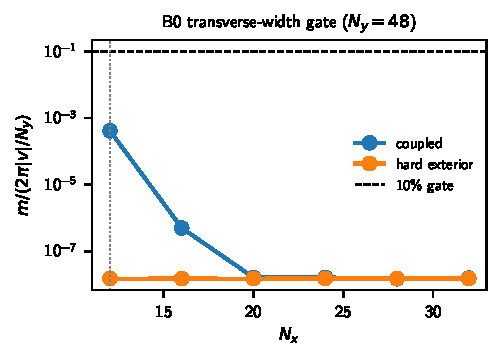
\includegraphics[width=0.48\textwidth]{../figures/width_convergence.pdf}
\caption{Transverse-width gate.  A failed gate is retained as a failed result rather than
changing the threshold.}
\end{figure}

\section{Entropy accounting}
The full-width strip has two entanglement boundaries and intersects both physical domain
walls.  Each three-column physical-wall contour window includes both entanglement cuts.
Those window sums are diagnostic contributions to the full entropy, not isolated subsystem
entropies.  The saved products test equality of the contour sum and the entropy, equality
of the two wall slopes, and the factor-of-two relation between a wall-window slope and the
full-strip slope.

\section{Acceptance ledger}
\begin{longtable}{p{0.36\textwidth}p{0.10\textwidth}p{0.46\textwidth}}
\toprule
requirement & status & details \\
\midrule
small-system formula and gauge preflight & PASS & completed before production stages \\
fixed-rank half filling & PASS & every geometry must contain exactly Nx Ny occupied orbitals \\
Hermiticity, projector, and contour numerics & PASS & absolute tolerance 1e-10 \\
transverse-width hybridization gate & PASS & selected Nx=12; ratio threshold 0.1 \\
coupled: opposite, compatible spectral velocities & PASS & v0=-0.990726, v1=0.990726, relative mismatch=3.36e-16 \\
coupled: finite transverse localization lengths & PASS & xi0=0.293039, xi1=0.293039 \\
coupled: Renyi q=1,2,3 full-strip c=1 & PASS & q=1: c=0.99956, q=2: c=0.99586, q=3: c=1.0005 \\
coupled: single-physical-wall contour factor of two & PASS & relative errors=[8.730643320187248e-05, 8.730643312238051e-05]; each window includes both entanglement cuts \\
coupled: wall squared-correlator exponent two & FAIL & betas=[2.341081443548334, 2.3410814435133576]; all four candidate models remain in correlator\_fits.csv \\
coupled: physical response chirality & PASS & response velocities=[-0.8720279720279717, 0.8720279720279717]; spectral velocities=[-0.9907263837597542, 0.9907263837597539]; relative magnitude errors=[0.11980947886068032, 0.11980947886068002] \\
coupled: response linearity and charge conservation & PASS & charge drift=3.7e-16; epsilon relative error=5e-07 \\
coupled: opposite modular packet velocities & FAIL & modular velocities=[0.0011550506430308726, 0.01806554891705961] \\
coupled: nonsingular overlap tracking & PASS & minimum singular value=0.714132 \\
coupled: unit wall flow and zero net flow & PASS & signed flows=[-1, 1] \\
hard\_exterior: opposite, compatible spectral velocities & PASS & v0=-0.990726, v1=0.990726, relative mismatch=5.6e-16 \\
hard\_exterior: finite transverse localization lengths & PASS & xi0=0.222754, xi1=0.222754 \\
hard\_exterior: Renyi q=1,2,3 full-strip c=1 & PASS & q=1: c=1.0001, q=2: c=0.99591, q=3: c=0.99333 \\
hard\_exterior: single-physical-wall contour factor of two & PASS & relative errors=[8.9031440549725e-05, 8.903144038829858e-05]; each window includes both entanglement cuts \\
hard\_exterior: wall squared-correlator exponent two & PASS & betas=[2.0743680296808296, 2.074368029466904]; all four candidate models remain in correlator\_fits.csv \\
hard\_exterior: physical response chirality & PASS & response velocities=[-0.8720279720279717, 0.8720279720279717]; spectral velocities=[-0.9907263837597533, 0.9907263837597539]; relative magnitude errors=[0.11980947886067952, 0.11980947886068002] \\
hard\_exterior: response linearity and charge conservation & PASS & charge drift=2.57e-16; epsilon relative error=5e-07 \\
hard\_exterior: opposite modular packet velocities & FAIL & modular velocities=[0.00954704076039757, 0.007104095358116392] \\
hard\_exterior: nonsingular overlap tracking & PASS & minimum singular value=0.999999 \\
hard\_exterior: unit wall flow and zero net flow & PASS & signed flows=[-1, 1] \\
33/65/129-point, both-sign, seam-relocation twist validation & PASS & all validation rows require unit absolute wall flow and seam/uniform spectral agreement \\
\bottomrule
\end{longtable}
The machine-readable ledger retains the same decisions and their thresholds.  Any failed
item remains explicit rather than changing the estimator or gate.
\end{document}
